\section{Materials and methods}\label{sec:methods}

This is a measurement study rather than a detector proposal. We do not train a new model for the central claim; we freeze two publicly specified detectors, run them through standard overlapping sliced inference, and instrument the pipeline so that every missed ground-truth object is charged to the stage that first removed it. The apparatus is therefore a bookkeeping ledger over a frozen candidate set, and the only quantities estimated are category proportions on a pre-registered audit set. All design choices below were frozen and hashed before any detector output on the audit set was inspected, and are listed in full in Table~\ref{tab:config}; the authors confirm that no frozen quantity was retuned on the audit set after the results were seen.

\subsection{Datasets, and the separation of size from frequency}\label{sec:data}

The primary dataset is RicePest-30~\citep{mo2025ricepest}, a 30-class detection set of 7{,}915 training and 933 validation images (62{,}227 boxes) combining ultraviolet light-trap captures, web imagery and laboratory close-ups, released under CC~BY-NC~4.0. Images are published at a long edge of at most 640\,px while boxes are stored in the original frame; we rescale each box per axis into the 640 frame and treat that frame as the reference throughout, so an object's size label is a property of the published image a practitioner actually feeds to a detector. We rank classes by training-set instance count and cut the ranking into head, middle and tail tertiles, and we call an object \emph{small} when its box area is below $32^2$ in the 640 frame, following the COCO convention. A separate group of 343 single-pest close-ups (300 training, 43 validation) records a JSON frame whose aspect ratio differs from the JPEG, so their boxes cannot be mapped; we exclude these and list them rather than dropping them silently.

Separating size from frequency matters because the folk rationale for slicing runs tail $\rightarrow$ small $\rightarrow$ cut by a tile boundary $\rightarrow$ lost, and the first link is already wrong here. Small objects are not concentrated in the tail: head classes carry a \emph{larger} fraction of small objects than tail classes do, so rarity and smallness are distinct axes that must be held apart before any loss is attributed to either (Fig.~\ref{fig:size-frequency}). The left panel places one point per class in the plane of training frequency against the fraction of that class smaller than $32^2$; the tail tertile is spread across the full range of small-fractions, and the single largest tail point is the leafhopper \textit{Jacobiasca formosana}. The right panel shows that each stratum's size composition is similar in the training and audit splits, so the strata are comparable across the split we evaluate on. This dissociation is the reason every subsequent analysis reports results at matched size rather than pooling across sizes.

\begin{figure}[!htbp]
    \centering
    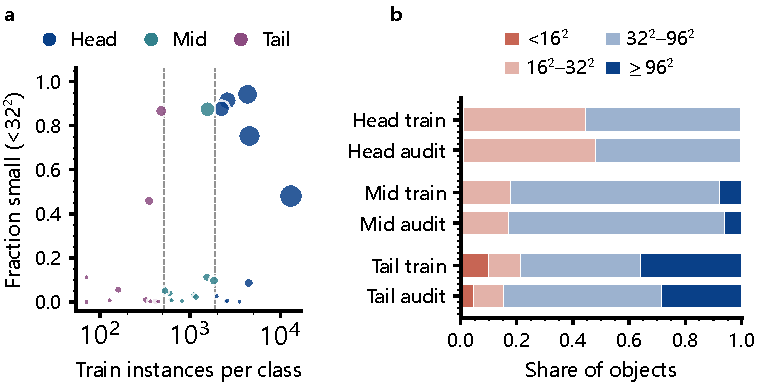
\includegraphics[width=0.98\textwidth,height=0.8\textheight,keepaspectratio]{../figures/fig_size_frequency.pdf}
    \caption{Size is a class property, not a frequency property (RicePest-30, 640-long-edge frame). Left: one point per class, training instances versus the fraction of its objects smaller than $32^2$; point area grows with the number of small objects of that class in the audit set; dashed lines separate the head, mid and tail tertiles. The large tail point is \textit{Jacobiasca formosana}. Right: size composition of each stratum in the training set and in the audit set.}
    \label{fig:size-frequency}
\end{figure}

The second dataset, Yellow Sticky Traps (YST) in its relabelled form~\citep{deserno2021relabeled}, is used only as a native-resolution source re-check: 284 images at $5184\times3456$ with 8{,}114 boxes across three classes under CC0. With three classes and an $8.4\times$ imbalance it is not long-tailed, and we draw no long-tail conclusion from it; its role is to test whether the stage at which objects are lost depends on the image source, at a resolution an order of magnitude larger than downscaled RicePest-30.

\subsection{A group-disjoint audit set, and the leakage it corrects}\label{sec:audit}

The published RicePest-30 split cannot support a tail claim as released, because many validation images recur in training. We link two images when their 64-bit perceptual hashes are within Hamming distance $\tau$ and they share a class, or when their files are byte-identical (MD5), and we take connected components as acquisition/dedup groups. At face value 285 of the 933 validation images have a training image at perceptual-hash distance 0, and 279 byte-identical groups straddle the split. We fix $\tau=8$ before unblinding and define the \emph{audit set} as the validation images whose component contains no training image: 367 of 890 frame-consistent validation images are discarded as contaminated, leaving 523 images in 508 groups with 4{,}429 objects, of which 38 (in 27 groups) are the tail-small endpoint. The threshold is a compromise between two failures that pull in opposite directions: too loose a threshold deletes genuine tail images and weakens the very stratum under study, the risk emphasised by the IP102-TailDet tail-completion benchmark~\citep{nguyen2026ip102taildet}, while too tight a threshold leaves near-duplicates across the split. Table~\ref{tab:leakage} reports the audit set at $\tau \in \{0,4,6,8,10,12\}$ so the reader can see this trade-off directly; the tail-small count falls from 43 to 22 across that range and sits at 38 at the frozen setting.

\begin{table}[!htbp]
\small
\caption{Train/validation near-duplicate grouping and the resulting group-disjoint audit set (RicePest-30, 890 frame-consistent validation images).}
\label{tab:leakage}
\begin{tabular*}{\textwidth}{@{\extracolsep{\fill}}rrrrrrr}
\toprule
$\tau$ & \shortstack{Contam.\\val} & \shortstack{Audit\\images} & \shortstack{Audit\\groups} & \shortstack{Head-\\small} & \shortstack{Mid-\\small} & \shortstack{Tail-small\\(groups)} \\
\midrule
0 & 249 & 641 & 626 & 1856 & 146 & 43 (30) \\
4 & 274 & 616 & 601 & 1854 & 146 & 43 (30) \\
6 & 315 & 575 & 559 & 1797 & 136 & 42 (29) \\
8$^{\ast}$ & 367 & 523 & 508 & 1686 & 114 & 38 (27) \\
10 & 444 & 446 & 431 & 1494 & 81 & 28 (21) \\
12 & 555 & 335 & 325 & 1097 & 49 & 22 (17) \\
\bottomrule
\end{tabular*}
\footnotetext{$\tau$: 64-bit pHash Hamming threshold for a near-duplicate link (links also require a shared class; byte-identical files are always linked). $^{\ast}$Frozen setting. 285 of 933 validation images have a training image at pHash distance 0; 279 byte-identical (MD5) groups span both splits.}
\end{table}


Evaluating on the contaminated split is not a harmless convenience. Running the same frozen pipeline on the discarded, contaminated validation images recovers 81.7\% of tail objects (93 objects), against 53.6\% on the group-disjoint audit images (248 objects); for head classes the gap is far smaller (85.7\% versus 82.4\%) and for all objects it is 84.1\% versus 79.3\% (Fig.~\ref{fig:leakage}). Near-duplicate leakage therefore inflates apparent tail recall by about 28 percentage points while barely touching head recall, the pattern expected when rare classes recur as near-identical images across the split. The leakage finding is itself a methodological result: any tail-recall number read off the published split is optimistic by roughly this margin, and the audit that follows is run only on the group-disjoint remainder.

\begin{figure}[!htbp]
    \centering
    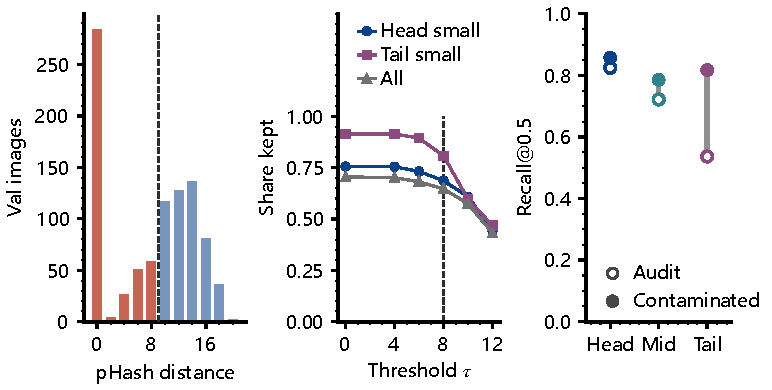
\includegraphics[width=0.98\textwidth,height=0.8\textheight,keepaspectratio]{../figures/fig_leakage.pdf}
    \caption{Leakage in the published split. Left: perceptual-hash distance from each validation image to its nearest training image (red at or below the frozen threshold $\tau=8$). Middle: share of validation objects kept in the group-disjoint audit set as $\tau$ varies. Right: recall@0.5 of the frozen pipeline on audit images (hollow) and on contaminated validation images (filled), per stratum.}
    \label{fig:leakage}
\end{figure}

\subsection{Frozen detectors and the per-tile candidate dump}\label{sec:detectors}

The primary detector is YOLO11n, a current one-stage anchor-free member of the YOLO family~\citep{redmon2016yolo}, fine-tuned from COCO initialisation for 60 epochs at input size 640 with batch 16 and a single training seed; the last checkpoint is taken with no selection on validation data, so no audit image influences the weights. A second detector, FCOS-ResNet50-FPN~\citep{tian2019fcos}, is fine-tuned for 6 epochs under an otherwise standard recipe and used only as a cross-detector check; it is deliberately undertrained, which we treat as informative about how the loss profile depends on the detector rather than as a competitive baseline. Both detectors and every geometric and read-out quantity are listed in Table~\ref{tab:config}, which is a verbatim copy of the frozen configuration file.

\begin{table}[!htbp]
\scriptsize
\caption{Frozen configuration, fixed and hashed before any detector output on the audit set existed.}
\label{tab:config}
\begin{tabular}{lp{0.72\linewidth}}
\toprule
Component & Setting \\
\midrule
Detector A & YOLO11n, COCO init, 640 input, 60 epochs, batch 16, seed 0, last checkpoint (no selection on validation) \\
Detector B & FCOS-ResNet50-FPN (torchvision), COCO init, 640, 6 epochs, batch 4, last checkpoint \\
Reference frame & image resized to 640-pixel long edge; size bins on box area in this frame \\
Views & full image + SAHI tiles $T$=320, overlap 0.25 (stride 240); every view letterboxed to 640 \\
Candidate dump & per-view score floor 0.01, per-view NMS IoU 0.7, max 300 boxes; single label per anchor \\
Read-out (merge) & SAHI GREEDYNMM, IOS 0.5, class-aware, on the floor-level dump \\
Operating point & score $\geq$0.25, at most 100 boxes per image; matching IoU $\geq$0.5, one-to-one \\
Grouping & 64-bit pHash, Hamming $\leq$8 with a shared class, or identical MD5; connected components \\
Audit set & validation images whose component holds no training image \\
Statistics & cluster percentile bootstrap over audit groups (2,000), Holm over 3 categories, class-label permutation (10,000) \\
Weights hash & YOLO11n bcde46c946b0; FCOS f41271c04f8e \\
\bottomrule
\end{tabular}
\end{table}


Sliced inference follows the SAHI protocol~\citep{akyon2022sahi}: each image is covered by $320\times320$ tiles at stride 240 (overlap 0.25) together with the full-image view, every view is run at a permissive 0.01 score floor, and the per-view boxes are merged by SAHI's class-aware greedy non-maximum-merging. For the primary dump this yields 113{,}489 standard candidates over the 890 validation images before merging, 43{,}603 merged boxes and 11{,}310 emitted at the operating point. Two sanity checks guard the dump. First, replaying our merge code on 80 real candidate lists reproduces SAHI~0.14.0's own greedy-NMM and NMS outputs exactly, with no count, class or score mismatch and a maximum coordinate difference of zero, so the ledger reads the same boxes a SAHI user would see. Second, candidate recall at the floor (94.8\% of audit objects) is at least the merged recall (89.1\%), which is at least the emitted recall (79.3\%), confirming that the dump loses nothing the later stages do not. For context, sliced inference reaches an AP@0.5 of 0.570 on the audit set against 0.607 for the full image alone, so on these downscaled images slicing helps small-object recall at the operating point (the score threshold and output cap at which detections are emitted, defined in Table~\ref{tab:config}) without raising average precision; this is the regime we audit.

\subsection{The per-object stage ledger}\label{sec:ledger}

The instrument traces each ground-truth object through five stages in the order the pipeline applies them: tile coverage (does any view hold the whole object), candidate formation (does any per-tile box at the floor match it), cross-tile merge/read-out, the score threshold, and the per-image output cap (Fig.~\ref{fig:arch}). An object is matched to a box by one-to-one assignment at IoU~$\geq 0.5$, and a miss is charged to the first stage that removes it. One ordering choice is pre-registered: when the merge produces a union box that matches the object although no single candidate did, the object is credited with a surviving merged box and charged later rather than at candidate formation, so the no-candidate category is reserved for objects that truly never produced a matching box in any view. Failing the first stage, coverage, is literal truncation and serves as the negative control described in Section~\ref{sec:prereg}.

\begin{figure}[!htbp]
    \centering
    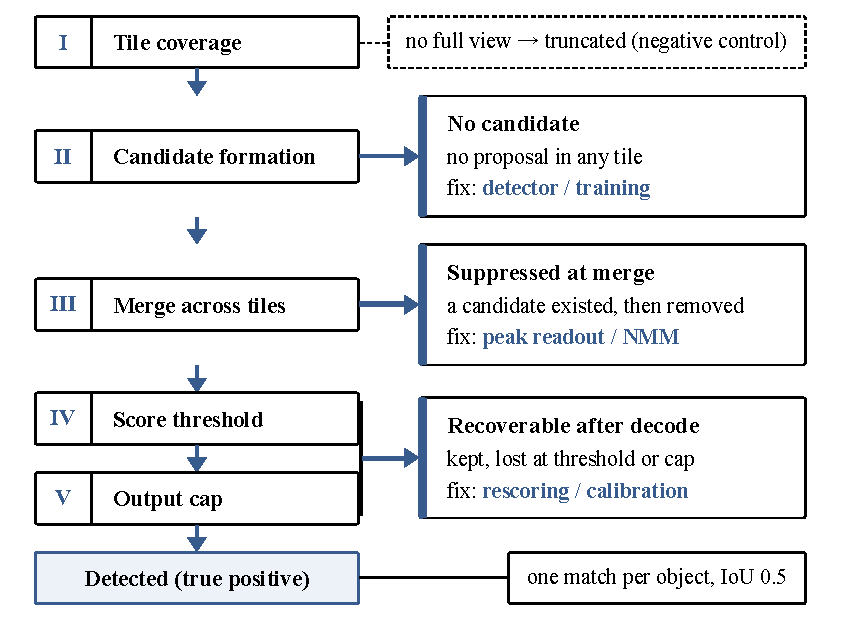
\includegraphics[width=0.92\textwidth,height=0.8\textheight,keepaspectratio]{../figures/fig_arch.pdf}
    \caption{The per-object stage ledger. An object traverses tile coverage, candidate formation, cross-tile merge, the score threshold and the output cap, and a miss is assigned to the stage that first removes it. The three recovery-ceiling categories (no candidate, suppressed before the scored list, recoverable after decoding) name the class of fix each miss admits; failing coverage is literal truncation, the negative control.}
    \label{fig:arch}
\end{figure}

\subsection{The recovery-ceiling partition}\label{sec:partition}

From the ledger we read a three-way partition of every missed object that states, for each miss, the most upstream intervention that could in principle recover it. A \emph{no-candidate} miss has no per-tile box at the floor within IoU~$0.5$ in any view; only a different detector or more training can reach it, because no amount of post-processing can resurrect a box that was never produced. A \emph{pre-suppression-only} miss did produce a per-tile box, but no merged box survives into the final scored list because the merge, the score threshold or the cap removed it; re-ranking the scored list cannot recover it, since the evidence is gone before the list is formed. A \emph{post-hoc-recoverable} miss keeps a merged box in the scored list but is not emitted at the operating point; score re-ranking, calibration or a larger cap can recover it. Naming these categories by the admissible fix is the point of the audit: locating a loss in one category rules an entire family of remedies in or out before any remedy is tried. The confirmatory endpoint is the proportion of pooled tail-small misses in each category, reported with absolute counts.

\subsection{An oracle full-view upper bound}\label{sec:oracle}

To bound how much a better read-out could ever recover without a new detector, we define an oracle that keeps every baseline detection and additionally admits each same-class candidate that scores at least the operating threshold in a view holding the whole object. This measures the headroom available to any read-out that reorders or re-selects the existing full-view evidence at fixed scores. A floor variant, which admits full-view same-class evidence down to the 0.01 floor, bounds instead what perfect rescoring of that evidence could reach. The gap between the two bounds separates what a smarter selection buys from what only a smarter score could buy, and the residual below both bounds is the no-candidate mass that neither can touch.

\subsection{Pre-registration, controls and statistics}\label{sec:prereg}

Every quantity in Table~\ref{tab:config}, the strata and size bins, the audit set and the statistical procedures were frozen before the final detectors produced any output on the audit set, which is what licenses reading the tail-small partition as confirmatory rather than selected after the fact. Two controls bound the measurement. The negative control is literal truncation under the frozen overlap: because an object with no full view in any tile cannot be detected at the candidate stage, a near-zero truncation rate is a precondition for attributing tail-small loss to anything downstream. The positive control removes the tile overlap, which must manufacture truncation if the instrument can see it at all; observing truncation reappear at overlap~0 confirms the measurement is not simply blind to the phenomenon.

Proportions are estimated with a cluster percentile bootstrap over audit groups (2{,}000 resamples), so that near-duplicate images resampled together cannot inflate precision; when a cell has fewer than 20 groups we add a leave-one-group-out range, and a pre-registered minimum-cell rule suppresses any rate or interval for cells below 10 events or 5 groups, leaving counts only. We chose the percentile and jackknife forms rather than the bias-corrected accelerated interval, which degenerates with few groups, while retaining the bootstrap as formalised by \citet{efron1987bca}. The size-matched frequency contrast re-weights head-small objects to the tail size mix and tests the difference by exact enumeration of all class-label permutations among the small-object classes, because a frequency label is a property of a class and cannot be permuted within a group. For the secondary read-out increment we test head precision with a one-sided paired cluster-bootstrap non-inferiority test at a 1-percentage-point margin; we cite \citet{schuirmann1987tost} only for the margin logic and do not perform two one-sided tests of equivalence. Holm correction controls the family of three primary categories and Benjamini--Hochberg the exploratory stage and size tables, with absolute counts beside every rate. The class-conditional read-out is declared positive only if it adds at least five tail-small true positives over class$\times$size calibration, passes head non-inferiority, and its tail-small recall interval excludes zero; otherwise it is reported as a negative increment. One limitation is fixed here by design: each detector is trained once, so the seed-to-seed variance of the partition is not estimated, and the single-seed caveat is carried through the results and discussion.




